% --- Header --- %
\documentclass[authoryear]{elsarticle}
\usepackage[utf8]{inputenc}
\usepackage{listings}
\usepackage{multirow}
\usepackage{geometry}
\usepackage{gensymb}
\usepackage{booktabs}
\usepackage{mathtools} 
\usepackage{lipsum}
\usepackage{color}
\usepackage{graphicx}
\usepackage{ragged2e}
\usepackage{pgfplots}
\graphicspath{ {figures/} }
\bibliographystyle{elsarticle-harv}
\usepackage{pgfplots}
\usepgfplotslibrary{statistics}

% --- PGF Plot Settings --- %
\pgfplotsset{
    box plot/.style={
        /pgfplots/.cd,
        black,
        only marks,
        mark=-,
        mark size=1em,
        /pgfplots/error bars/.cd,
        y dir=plus,
        y explicit,
    },
    box plot box/.style={
        /pgfplots/error bars/draw error bar/.code 2 args={%
            \draw  ##1 -- ++(1em,0pt) |- ##2 -- ++(-1em,0pt) |- ##1 -- cycle;
        },
        /pgfplots/table/.cd,
        y index=2,
        y error expr={\thisrowno{3}-\thisrowno{2}},
        /pgfplots/box plot
    },
    box plot top whisker/.style={
        /pgfplots/error bars/draw error bar/.code 2 args={%
            \pgfkeysgetvalue{/pgfplots/error bars/error mark}%
            {\pgfplotserrorbarsmark}%
            \pgfkeysgetvalue{/pgfplots/error bars/error mark options}%
            {\pgfplotserrorbarsmarkopts}%
            \path ##1 -- ##2;
        },
        /pgfplots/table/.cd,
        y index=4,
        y error expr={\thisrowno{2}-\thisrowno{4}},
        /pgfplots/box plot
    },
    box plot bottom whisker/.style={
        /pgfplots/error bars/draw error bar/.code 2 args={%
            \pgfkeysgetvalue{/pgfplots/error bars/error mark}%
            {\pgfplotserrorbarsmark}%
            \pgfkeysgetvalue{/pgfplots/error bars/error mark options}%
            {\pgfplotserrorbarsmarkopts}%
            \path ##1 -- ##2;
        },
        /pgfplots/table/.cd,
        y index=5,
        y error expr={\thisrowno{3}-\thisrowno{5}},
        /pgfplots/box plot
    },
    box plot median/.style={
        /pgfplots/box plot
    }
}

% --- BEGIN Document --- %
\begin{document}

% --- BEGIN Front Matter --- %
\begin{frontmatter}

\title{A system for integrating computer-vision guidance with inter-row cultivator
  implement feedback}
\author[rvt]{Trevor Stanhope}
\ead{trevor.stanhope@mail.mcgill.ca}
\author[rvt]{Viacheslav Adamchuk}
\ead{viacheslav.adamchuk@mail.mcgill.ca}
\author[els]{Jofroi Desperrier-Roux}
\ead{jofroi-desperrier@agrifusion.ca}
\address[rvt]{McGill University, 21111 Lakeshore Road,
  Sainte-Anne-de-Bellevue, Quebec, Canada}
\address[els]{Agri-Fusion 2000, Inc., 481 Chemine Saint Philippe,
  Saint-Polycarpe, Quebec, Canada}

\begin{abstract}
Management of organic row crops requires frequent in-field
operations. Depending on the degree of soil conservation practices, 
weed control necessitates tillage operations. Strip-tillage and
cultivator implements require precise guidance systems to
assure proper positioning of the working tools. Legacy systems have
made use of mechanical guiding rods, however such
systems perform poorly during the earliest stages of crop growth.
Modern techniques based on RTK GPS are available commercially but are
prohibitively expensive for small-scale operations.
Therefore, the objective of this study was to develop a low-cost CCD 
camera system which is capable of supplementing the mechanical row
detection during inter-row cultivation.
A computer-vision guidance system was developed for the Intel Atom 
architecture to interface with an electro-hydraulic steering hitch system.
Two redundant CCD cameras were mounted to the cultivator toolbar
in-line with crop rows to obtain a video stream of the plants passing
beneath the implement. The OpenCV platform was used to develop an
algorithm for identifying the lateral offset of the plant rows and
adjust the hydraulic steering accordingly via PID control. The
computer-vision guidance system was tested successfully without GPS
RTK assistance at travel speeds of 6, 8, 10, and 12 km/h in corn and
soybean fields under varying ambient light and crop conditions.
\end{abstract}

\begin{keyword}
\texttt{Computer-vision, inter-row cultivation, control systems}
\end{keyword}

\end{frontmatter}
% --- END Front Matter --- %

% --- BEGIN Introduction --- %
\section{Introduction}
Unlike conventional farming where herbicide application is the primary
method for weed prevention, organic farmers must use tillage
implements such as inter-row cultivators. Inter-row cultivation is a
field operation which requires precise control of the implement in
order to maximize the tillage area without causing damage to the
crops. Cultivation is often conducted at speeds of up to 12 km/h with
an error tolerance of only $\pm$5 cm. Although many organic farmers are equipped
with RTK-level global navigation satellite systems (GNSS) for tractor
steering, such systems are uncommon and expensive for guiding tillage
implements. As such, many farmers prefer to use older,
mechanically-guided tillage systems. A common method for
mechanically-guided cultivators employs guiding rods (also known as
brushes) which are mounted to a rotating voltage divider
(\ref{guiding_rods}). These rods make contact with the crop stems and
their position approximates that of the crop row. The resulting reference
signal is fed to a hydraulic control system which adjusts the steering
mechanism of the implement accordingly. Although these
mechanically-guided systems are rugged and maintainable, the guiding
rods perform poorly with seedlings. During the early stages of growth
(e.g. $\le$15 cm), guiding rods have the potential to cause damage to
the crop or lose track of the row, forcing operators to travel at
speeds of less than 6 km/h. To address this issue, modern systems
implement non-contact detection methods, such as a secondary RTK GNSS
antennae or cameras, to estimate the lateral offset of the cultivator.

\begin{figure}
  \centering
  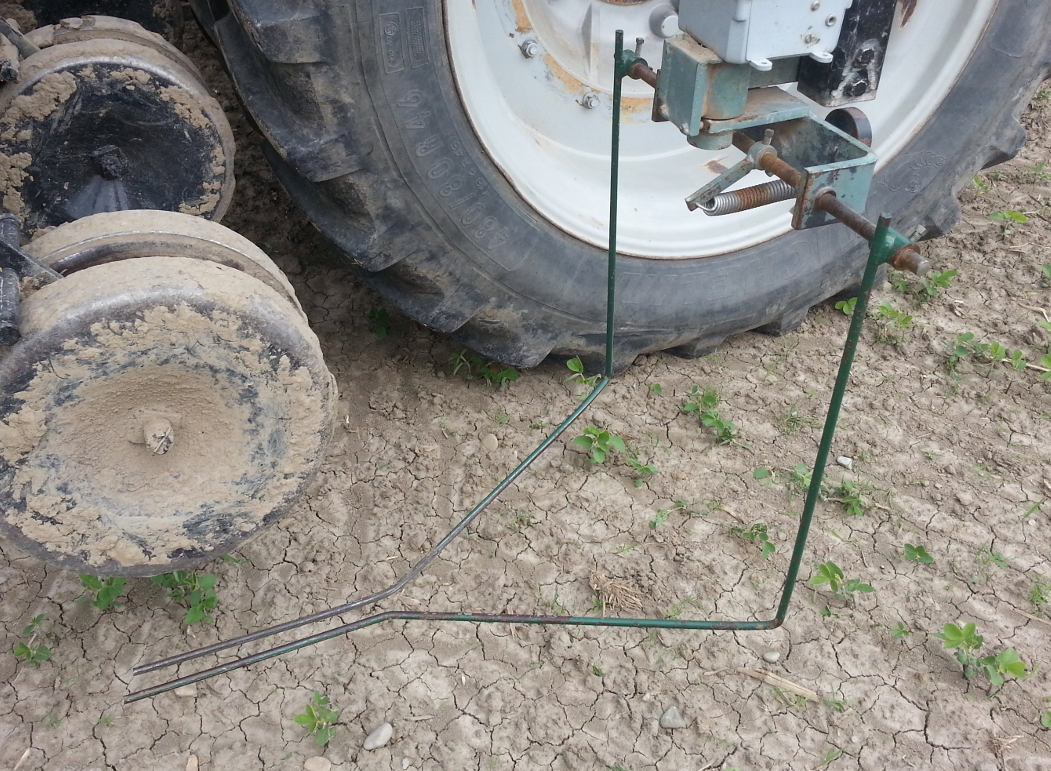
\includegraphics[width=0.8\textwidth,natwidth=610,natheight=642]{guiding_rods.jpg}
  \caption{Mechanical guiding rods.}
  \label{fig:guiding_rods}
\end{figure}

The objective of this study was to develop a low-cost embedded system
which extends computer-vision row detection functionality to existing
electro-hydraulic implement guidance systems. To be considered
effective for commercial use, such a guidnace system must be capable
of 4 cm precision 95 percent of the  time for travel speeds up to 12
km/h and for crops up to 20 cm in height.
% --- END Introduction --- %

% --- BEGIN Literature Review --- %
\section{Literature Review}
Demand for high-precision tractor control has produced significant
research interest over the past two decades. In addition to advances
in global navigation satellite system (GNSS) guidance systems,
research has demonstrated that computer-vision systems can be
implemented to detect the lateral offset of the crop rows relative to
the tractor/implement with a high degree of reliability and accuracy.
By integrating computer-vision systems into agricultural platforms,
the precision of field operations can be improved. Research applications of
computer-vision row detection have demonstrated that computer-vision
guidance systems can be an effective approach for feedback and
control of agricultural implements. Several different computer-vision
methodologies have been proposed for identifying the position of the
crop rows, including stereo-vision, Hough Line Transform, and band-pass
analysis, among others. The predominant challenge is the
determination of the distribution of plant foliage within the
captured images and the subsequent differentiation between the crop
row and soil/weeds, a process known as segmentation.

% On color indices ...
With respect to the segmentation of green vegetation (e.g. for
crop-row tracking or weed detection), a significant amount of research
has been focused on developing robust color indices. Using unfiltered
RGB data is not employed due to the high correlation between the three
channels. Therefore, conversion to an alternate color index is often
advantagous for plant identification. Crop-specific color-indices have
been developed for agricultural application, such as Excess Green
(ExG) \citet{woebbecke1995} and Vegetative index (VEG)
\citep{hague2006} have been proposed, while standard indices such
Hue-Saturation-Value (HSV) have also seen significant implementation
\citep{moorthy2015}. An approach proposed by \citet{meyer1998}
demonstrates a contrast filter known as Excess Green (ExG) calculated
using the following equation:  

\begin{equation}
    ExG = \displaystyle\sum_{j=1}^{H} \displaystyle\sum_{i=1}^{W}
    \frac{G_{i,j}-R_{i,j}}{R_{i,j} + G_{i,j} + B_{i,j}}
    \label{eq:excess_green}
\end{equation}
\begin{flushleft}
where $n_{x}$ = image width (pixels); $n_{y}$ = image height (pixels).
\end{flushleft}

% On the two big problems ...
During the process of crop detection, varying ambient light is one of
the major limiting factors for successfully implementing
computer-vision guidance for weed control. Variations in the ambient
light occur naturally with changes in weather and time of day, and can
dramatically change the appearane crop foliage, e.g. texture and
color, in a digital image. Additionally, non-uniform lighting
intensity, e.g. shadows cast by the agricultural, are also a major
concern. Non-uniform lighting results in irregular variance in the
intensity of pixels and thus increases the complexity of segmenting
plants using color-indices. 

\begin{figure}
  \centering
  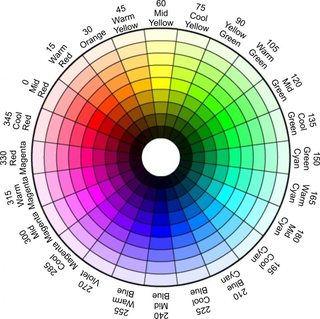
\includegraphics[width=0.8\textwidth,natwidth=610,natheight=642]{hsv.jpg}
  \caption{HSV Transform (360 degree).}
  \label{fig:hsv}
\end{figure}

% On thresholding ...
Therefore, a necessary component of robust segmentation algorithms
is the proper selection of threshold values to binarize the
color-index image. Thresholding techniques proposed to 
segment crop images include dynamic thresholding method
\citep{rovira2005}, Otsu-based thresholding methods \citep{meyer2008}
and statistical mean-based segmentation of the image
\citep{guijarro2011}. Although functional, these methods generally
assume the histogram of the image to be bimodal and require the
vegetation and background to belong to two different brightness regions.

% On learning ...
However, although thresholding reduces errors due to varying ambient
lighting, typically such methods experience reduced performance due to
non-uniform illumination conditions. In recent years,
research has been carried out on developing complex, yet efficient,
algorithms for vegetation segmentation. Examples of such techniques
include mean-shift-based learning procedure \citep{zheng2009},
Environmentally Adaptive Segmentation Algorithm (EASA)
\citep{tian1998}, and a Naive Bayes learner using HSV, G-R and
normalized RGB \citet{moorthy2015}.  

% On row detection ...
After segmentation of the plants within the image, it is necessary to
determine the lateral offset of the crop row. Methods for determining
the lateral offset can be grouped into two classes based on whether
the camera’s angle of inclination is either equal to zero, or greater
than zero; these classes are referred to as orthogonal or perspective,
respectfully. 

\begin{figure}
  \centering
  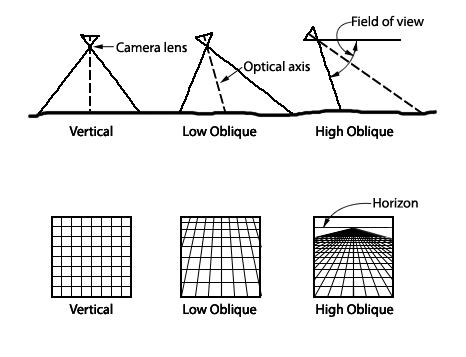
\includegraphics[width=0.8\textwidth,natwidth=610,natheight=642]{oblique_projection.jpg}
  \caption{Perspective vs. orthogonal viewing angles.}
  \label{fig:projection}
\end{figure}

% On orthogonal approaches ...
Orthogonal methods rely on a camera which faces vertically downward
and is directly aligned with a single crop row of the cultivator. A
basic approach proposed by \citet{olsen1995} for detecting the
lateral offset of the crop relies on taking the sum of the pixel
elements grey values in the direction of travel. The resulting curve
represents the likelihood of the row’s position for each x-index
within the image. To isolate the most probable offset, two separate
methods were compared: 1) a least squares regression of a sinusoidal
wave, and 2) a Fourier Fast Transform (FFT) low-pass filter. Both
filtration methods were effective in cereals to within an error of 10
mm, but performed poorly on sugar beets due to their
characteristically large leaf volume. In a similar study by \citet{slaughter1995}, an algorithm for detecting the lateral offset of the
row using individual segmentation of plants in the image was
proposed. For each plant, a histogram of the intensities was
calculated which was then used to find the median offset of each
plant. If a plant’s median was significantly different than the other
plants in the image, it was considered a weed and disregarded. The row
offset was then calculated based on the medians of the remaining
plants. This method was tested on lettuce and tomatoes for use with a
band sprayer operating at 8 km/h and performed successfully with
standard error of 9 mm and within 12 mm 95\% of the time.

% On perspective approaches ...
Conversely, perspective methods rely on a camera with a positive angle
of inclination with multiple rows in the field of view. One approach
for perspective guidance utilizes the Hough Line Transform (HLT)
algorithm to detect linear rows in cauliflower, sugar beets, and
wide-spaced wheat. In a study by \citet{pla1997}, a system using HLT
performed with an error of 18 mm, which was considered sufficient by
the researchers. A similar perspective approach using a band-pass
filter proposed by \citet{hague2001} based on
prior knowledge of the spacing of the crop rows was developed for use
on cereals and beets. Supported by the British Beet Research Organization the
developed system was capable of 3 cm precision at speeds of up to 10
km/h. The project was considered highly successful and was
commercialized in 2001 in partnership with Garford Farm Machinery and
Robodome Electronics under the name RoboCrop.

% On orthogonal vs perspective ...
When comparing the orthogonal and perspective methods, both have
advantages and disadvantages. The perspective approach is less
sensitive to missing plants and high weed density. However,
perspective methods rely on prior knowledge of the crop spacing and
linear rows with low curvature. Comparatively, orthogonal systems
optimize resolution, in pixels-per-centimeter, and require very only
basic calibration. Lens distortion is an issue for perspective
systems. To compensate for increased subject distance, perspective
methods require a higher resolution camera, resulting in greater
computational requirements and costs. The reduced field of view for
orthogonal systems is a concern when there are significant gaps in the
crop rows. To address the issues inherent to the orthogonal approach,
a system with two or more cameras may provide sufficient redundancy.

% On actuation ...
Actuation of the implement position can be achieved by several
methods, such as vehicular steering, pivoting hitches, side-shift
hitches, or stabilizer steering. Of these, vehicular steering has
received tremendous interest however is not applicable in all
environments. Some providers have produced mountable steering but no
computer-vision versions have been successfully produced. Pivoting
hitch systems have also been manufactured. For light cultivation, the
side-shift style hitch has been demonstrated to be effective. However,
this method causes problems when mounted to a heavy cultivator (deep
harrows or coulters) due to “jumping”, i.e. the effect of the hitch
shifting the tractor. To address this requires either removing tools
or dramatically increasing the weight of the tractor, both of which
are undesirable to the farmer. Stabilizer steering has applications in
heavier tillage.

\begin{equation}
  D = F_{i} \left[ A + B(S) + C(S^2) \right] W * d
  \label{eq:soil_resistance}
\end{equation}

A hydraulic hitch positional control system can be expressed as a
linear system. The output is the lateral error of the vehicle relative
to the crop row and the input is the position of the steering
mechanism. Additionally, state-information of the system is required,
and it is assumed the angular speed is constant and travel speed is
within acceptable bounds. To control this system, the voltage signal
to the electrohydraulic steering can be modulated to adjust the
lateral position of the cultivator.

\begin{equation}
  F_x = V - \rho\theta(sin \beta sin \alpha \sin \theta + cos \alpha +
  cos \theta)
  \label{eq:horizontal_velocity}
\end{equation}
\begin{flushleft}
where $V_x$ is the velocity in the x-axis, $\theta$ is the yaw of the
disc, $\alpha$ is the pitch of the
disc, $\beta$ is the roll of the disc, $\rho$ is the distance from
the axis of rotation of the disc to the given point of the working surface.
\end{flushleft}
% --- END Literature Review --- %

% --- BEGIN Methodology --- %
\section{Methodology}
For field evaluation, a twelve row Hiniker cultivator equipped with a
Sukup Auto-Guidance system mounted to a Fendt Vario 850 was used
throughout the testing period. The cultivator toolbar was configured
to a row-spacing of 30 inches. Steering actuation of the cultivator
was achieved via two 75 cm stabilizers mounted 165 cm behind the
cultivator toolbar and spaced 147.8 cm apart. The hydraulic actuation
of the stabilizers had maximum angular travel of $\pm$1.31 rad and angular
velocity of 0.4 rad/s.

\begin{figure}
  \centering
  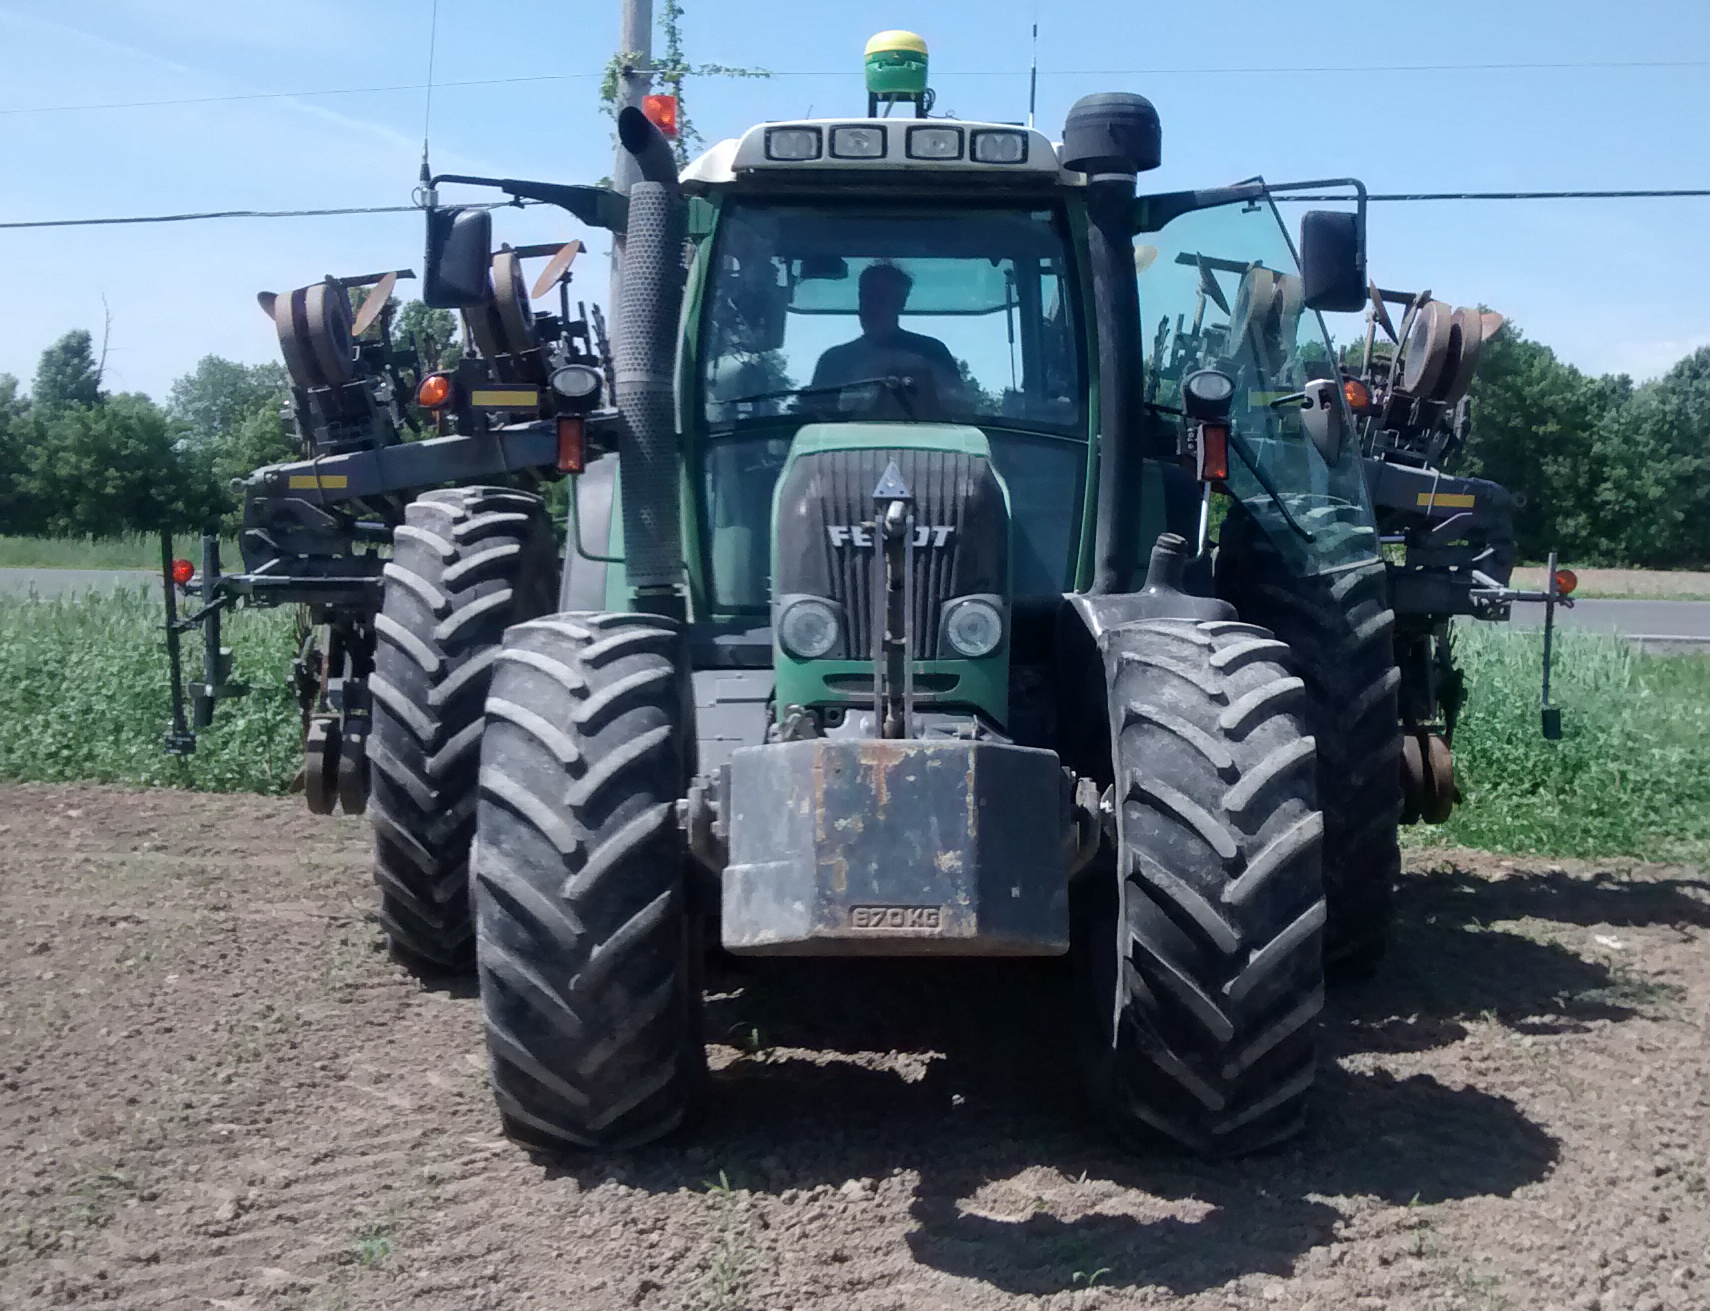
\includegraphics[width=0.8\textwidth,natwidth=610,natheight=642]{fendt_front.jpg}
  \caption{Diagram of the cultivator implement mounted to the tractor.}
\end{figure}

The computer-vision guidance system was installed alongside the
existing mechanical guidance system to act as a replacement for the
guiding rod potentiometer. The remaining components of the Sukup
Auto-Guide system, including the electrohydraulic controller,
center-pivot potentiometer, manual adjustment inputs, and hydraulic
solenoids, were unmodified. This configuration allowed easily
switching between the two modes of operation during field trials.

\begin{figure}
  \centering
  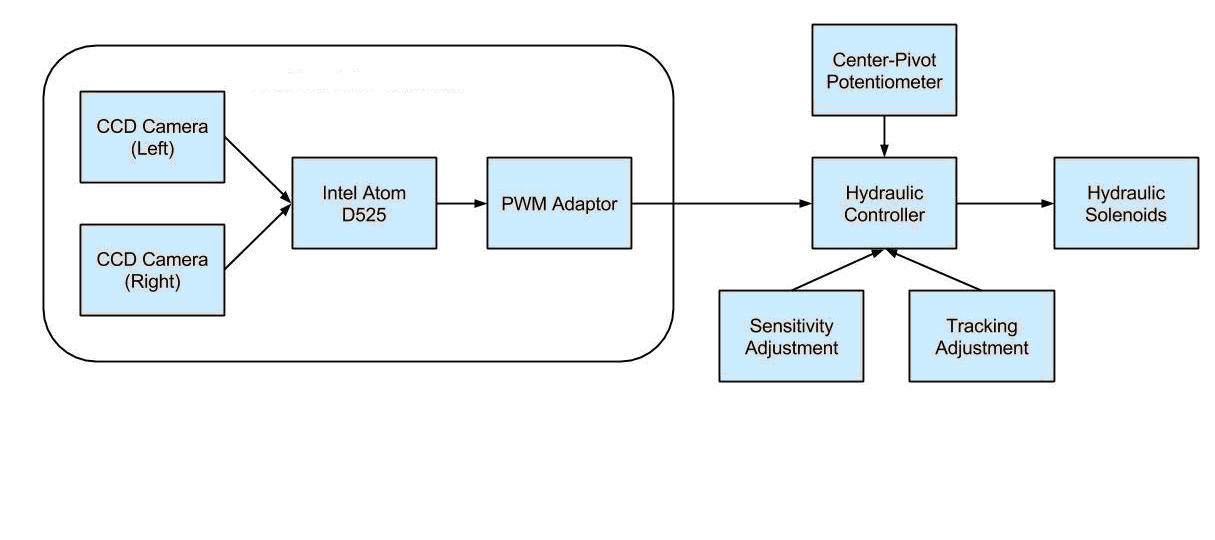
\includegraphics[width=0.8\textwidth,natwidth=610,natheight=642]{agcv_diagram.png}
  \caption{Diagram of the computer-vision system integrated with hydraulic controller.}
\end{figure}

Images of the plants passing beneath the cultivator are captured by
two weather-proof CCD cameras mounted via C-brackets to he toolbar. 
In a compromise between the orthogonal and perspective
methods, the two cameras were mounted at a 30$^{\circ}$ inclination from
vertical and a subject depth of 100 cm. This approach provides
additional longitudinal field of view without significantly
contributing to image distortion. To provide row estimation redundancy
in the event of regions of high weed density or gaps in the crop rows,
the two cameras were installed on the 3rd and 9th row of the
cultivator.

An embedded Linux system based on the Debian 7.8 operating system
(Linux Kernel 3.2) was developed for the Intel Atom D525
architecture. A 1.8GHz processor was used, with a 32 GB SSD, and 1 GB
of RAM (Jetway). A run-time application was developed for the system
using the Python programming language (v. 2.7.6) which operated as a
local microwebserver. A high-speed database server (MongoDB 32-bit)
was implemented for ultra-low latency storage and retrieval of
data. This robust platform provided sufficient computing power for
real-time image analysis at a relatively low cost. To generate the
output voltage signal of the control system, an
ATmega328P microcontroller was implemented as an 8-bit PWM generator. The
microcontroller was integrated as a Universal Serial Bus (USB)
peripheral device with the microprocessor serving as the
host. Lastly, a graphical user interface was developed in order to provide a
live video feed for the operator.

\subsection{Plant Segmentation}
Video of the crop rows were captured in real-time from the two CCD
cameras. The cameras used for this study had a native resolution and
frame-rate of 640x480 and 25 frames-per-second, respectively. However,
were hardware downscaled to a resolution of 320x240 and 16
frames-per-second. After capturing an image, the image matrix was
transformed from the Red-Green-Blue (RGB) color-space to the
de-correlated Hue-Saturation-Value (HSV) color-space in order to
simplify band-pass filtering operations (Equations \ref{eq:rgb2h} to \ref{eq:rgb2v}).

\begin{equation}
  H_{i,j} =
  \begin{cases}
    60 * \frac{G-B}{V_{i,j}-min(R_{i,j},G_{i,j},B_{i,j})} & \quad \text{if } V = R \\
    120 + 60 * \frac{B-R}{V_{i,j}-min(R_{i,j},G_{i,j},B_{i,j})} & \quad \text{if } V = G \\
    240 + 60 * \frac{R-G}{V_{i,j}-min(R_{i,j},G_{i,j},B_{i,j})} & \quad \text{if } V = B \\
  \end{cases}
  \label{eq:rgb2h}
\end{equation}

\begin{equation}
  S_{i,j} = 
  \begin{cases}
    \frac{V_{i,j}-min(R_{i,j},G_{i,j},B_{i,j})}{V_{i,j}}  & \quad \text{if } V \neq 0 \\
    0  & \quad \text{else}\\
  \end{cases}
  \label{eq:rgb2s}
\end{equation}

\begin{equation}
  V_{i,j} = max(R_{i,j},G_{i,j},B_{i,j})
  \label{eq:rgb2v}
\end{equation}

After transforming the image to the HSV color-space, a band-pass plant
detection filter (BPPD) was applied to isolate pixels which could
represent plant foliage. This filter selects for pixels with hue
ranging from yellow-green to blue-green, saturation above the mean
saturation, and value (i.e. brightness) between the extremes of under-
and over-exposed. Threshold values were determined empirically using a
training set of sample images in varying light and crop
conditions. During this process, it was observed that the cameras
experienced significant blue-shifting of crop foliage in very bright
or low light, so the upper threshold for hue was set well into the
cyan-blue region. This change did not have any noticeable negative
impact on performance due to the relative lack of blue-tones in soil.
\begin{equation}
  P_{n}(C) = A_{nN} + (nN \text{mod} 1) \times (A_{\lfloor nN \rfloor + 1}-A_{nN})
  \label{eq:percentile}
\end{equation}
\begin{flushleft}
where $n$ is the percentile of the  sorted array $A$ of $C$ of length N.
\end{flushleft}

\begin{equation}
BPPD_{i,j} =
  \begin{cases}
    1  & \quad \text{if } H_{min}<H_{i,j}<H_{max}(S) \bigwedge P_{k}(S)< S_{i,j} <P_{l}(S) \bigwedge P_{m}(V)< V_{i,j}<P_{n}(V)\text{ }\\
    0  & \quad \text{else}\\
  \end{cases}
  \label{eq:bppd}
\end{equation}
\begin{flushleft}
where $H_{min}=45$ (yellow-green), $H_{max}=105$ (blue-green).
\end{flushleft}

The BPPD filter utilizes the linear interpolation percentile function
to calculate the upper and lower thresholds of the Value and
Saturation bands. This approach eliminates the need for static limits,
reducing false-positive classification of pixels as green under
varying lighting conditions. As a final post-processing step,
morphological opening with a 3 by 3 kernel was applied to the BPPD
mask to reduce any remaining noise while preserving the structure of
crop foliage:

\begin{equation}
M = BPPD \otimes
\begin{bmatrix}
       1 & 1 & 1 \\
       1 & 1 & 1 \\
       1 & 1 & 1
     \end{bmatrix}
\label{eq:morph_opening}
\end{equation}
\begin{flushleft}
where K is a 3 by 3 kernel.
\end{flushleft}

This three step process is computationally non-intensive, yet produces
sufficient segmentation in diverse lighting conditions. Notably, the
percentile-based band-pass filters of saturation and intensity
produced reliable masks in scenarios of extreme exposure and shadows.

\begin{figure}
  \centering
  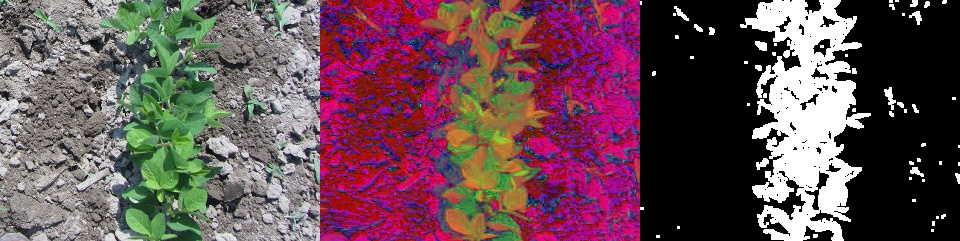
\includegraphics[width=0.8\textwidth,natwidth=610,natheight=642]{bppd_normal.jpg}
  \caption{BPPD applied to image of soy row.}
  \label{fig:bppd_normal}
\end{figure}

\begin{figure}
  \centering
  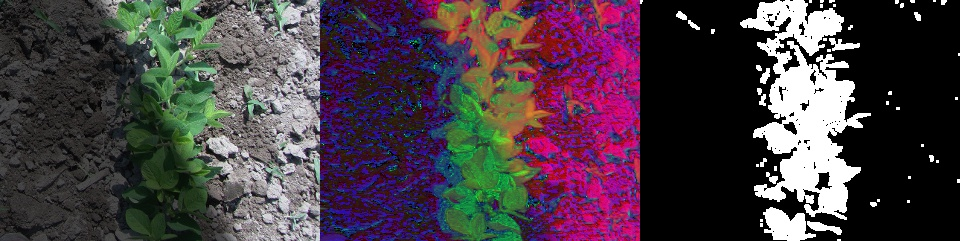
\includegraphics[width=0.8\textwidth,natwidth=610,natheight=642]{bppd_shadow.jpg}
  \caption{BPPD Shadow}
  \label{fig:bppd_shadow}
\end{figure}

\subsection{Row Estimation}
After the plant foliage mask (M) has been produced, the column
summation of the mask was calculated in the direction of travel,
resulting in an array (C) representing the lateral distribution of
plant foliage within the image. 

\begin{equation}
  C_{i} = \displaystyle\sum_{j=1}^{H} M_{i,j}
  \label{eq:col_sum}
\end{equation}
\begin{flushleft}
where H=240
\end{flushleft}

Indices of the C-array with low values suggest bare-soil, moderate
values suggest sparsely distributed weeds, and higher values suggest
presence of the crop row due to the longitudinal alignment of the
plant foliage. Using this distribution, the centroid of the crop row
was estimated by applying a high-pass filter to select for indices
which are significantly greater than others: 

\begin{equation}
  p_{i} =
  \begin{cases}
    i & \quad \text{if } C_{i} \geq P_{\alpha}(C) \\
    0 & \quad \text{else} \\
  \end{cases}
  \label{eq:p_threshold}
\end{equation}
\begin{flushleft}
where $\alpha$=0.95
\end{flushleft}

The array (p) consists of all indices of the image which are most
likely to represent the crop row. The estimated centroid of the crop
row was determined by taking the weighted mean of the probable
indices, where weight of each index was the normalized value of its
corresponding column summation:

\begin{equation}
    x = \frac{\displaystyle\sum_{i=1}^{N} p_{i} \times
      C_{i}}{\displaystyle\sum_{j=1}^{N} C_{p_{i}}} - \frac{W}{2}
  \label{eq:centroid}
\end{equation}
\begin{flushleft}
where $N$ is the number of elements in $p$ and $x$ is the position the
estimated centroid in pixels.
\end{flushleft}

To compensate for errors in the detection process inherent to single
camera systems, the row centroid estimation process was repeated for
each image, producing two column summation arrays ($C_{1}$ and $C_{2}$) and two
estimated row centroids ($x_{1}$ and $x_{2}$). After calculating the estimated
row centroid for each camera, the centroid and column summation values
are compared to determine the final estimated offset of the crop row:

\begin{equation}
  e = 
  \begin{cases}
    mean(x_{1},x_{2})  & \quad \text{if } |x_{1}-x_{2}| \leq  \epsilon\\
    argmax(C_{1},C_{2})  & \quad  \\
  \end{cases}
  \label{eq:camera_selection}
\end{equation}
\begin{flushleft}
where $\epsilon$ is the maximum acceptable error tolerance, $W$ is the width of
the camera in pixels. 
\end{flushleft}

This approach prioritizes centroid estimations which are in agreeance
and in the event of disagreeance between the two cameras the dominant
centroid was taken as the row. This provided a simplistic means for
reducing errors due to weeds. For the sake of performance evaluation,
the error in pixels may be converted to centimeters using the
relationship between the cameras’ field-of-view of 64 cm, measured
width-wise along the center-line, at a subject depth of 100 cm. For a
resolution of 320 px in width, this results in a resolution of 0.2 cm/px.

\begin{equation}
  x = \frac{We}{w}
  \label{eq:px2mm}
\end{equation}
\begin{flushleft}
where $e$ is the error, $W$ is the field-of-view of the camera (in
centimeters), $w$ is the camera width (in pixels).
\end{flushleft}

This is what it looks like:

\begin{figure}
  \centering
  % 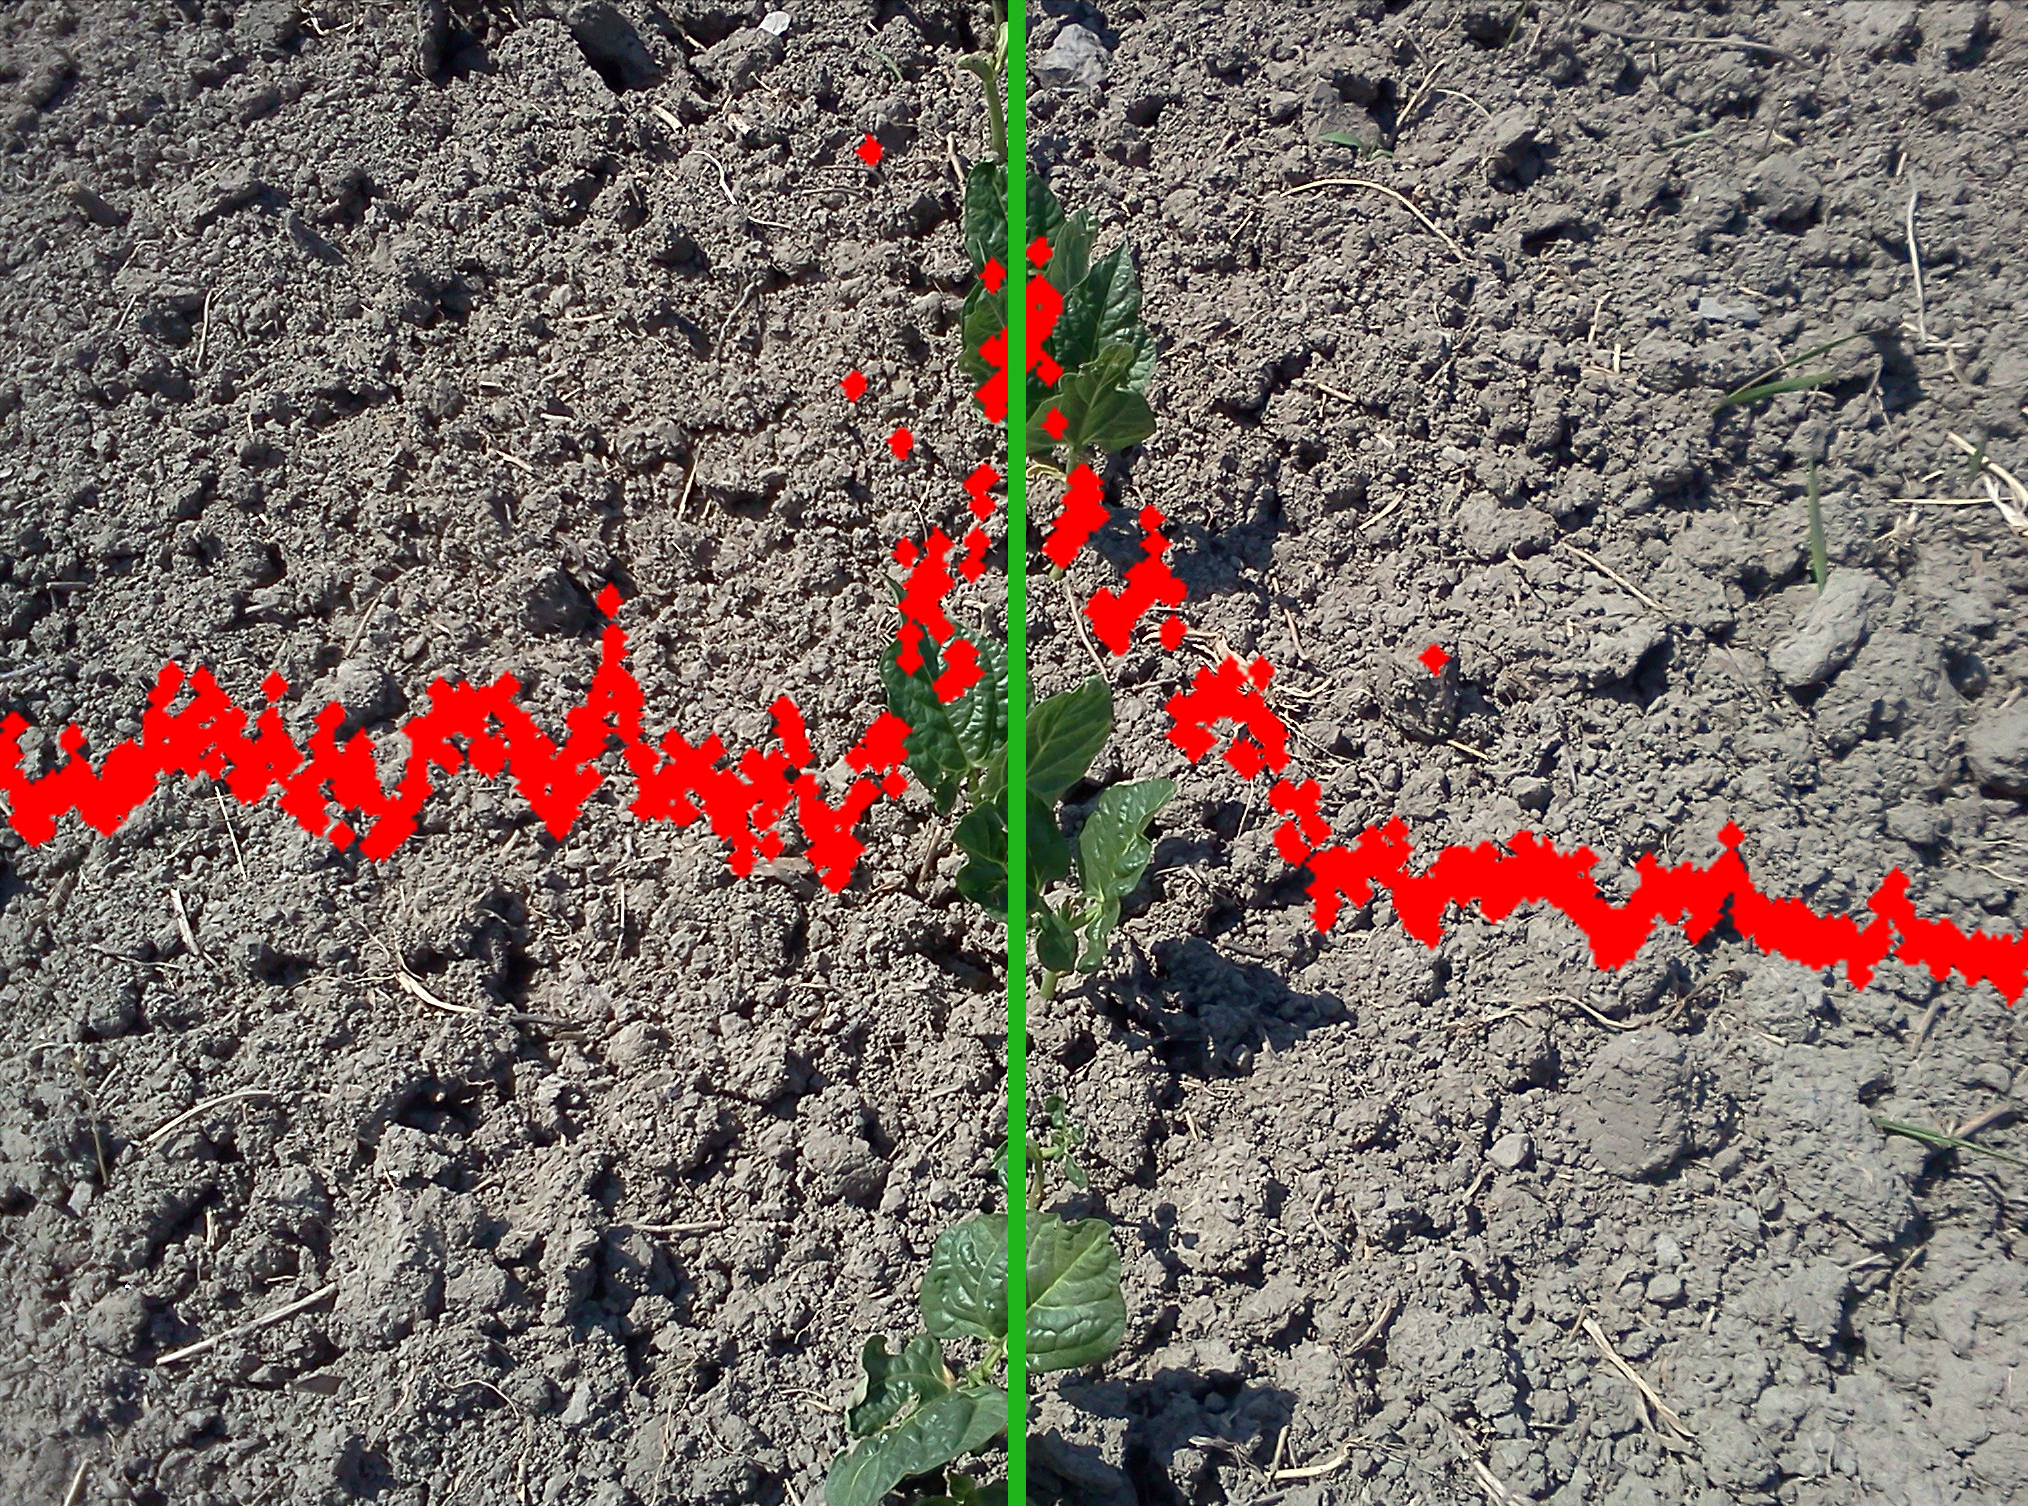
\includegraphics[scale=0.4]{row_estimation.jpg}
  \caption{Demonstration of offset detection.}
  \label{fig:row_estimation}
\end{figure}

\subsection{Electro-hydraulic Control}
The rotary stabilizer mechanism was operated via bang-bang hydraulic
solenoid controller whose actuation was based on the voltage
differential between the feedback signal from the row detection
system, i.e. the guiding rods or computer-vision module, and the
potentiometer mounted to the rotary mechanism on the hitch. 
To generate a smooth output signal, a signal conditioning based on a
Proportional-Integral-Derivative (PID) feed-back controller was
implemented. Coefficients were initially chosen to provide similar
response to that of the guiding rods and were subsequently modified by
trial and error.
\begin{equation}
    u(t) = K_{P}e_{t} + \frac{K_{I}}{N}\displaystyle\sum_i^N \left[
      e_{t-i} \right] +
    \frac{K_{D}}{M}\displaystyle\sum_{i=1}^M \left[e_{t-i}-e_{t-i-1}\right]
  \label{eq:pid}
\end{equation}
\begin{flushleft}
where $K_{P}=1.0$, $K_{I}=4.0$, $K_{D}=0.5$, $N=15$ is the number of integral samples,
$M=3$ is the number of differential samples.
\end{flushleft}

\begin{figure}
  \centering
  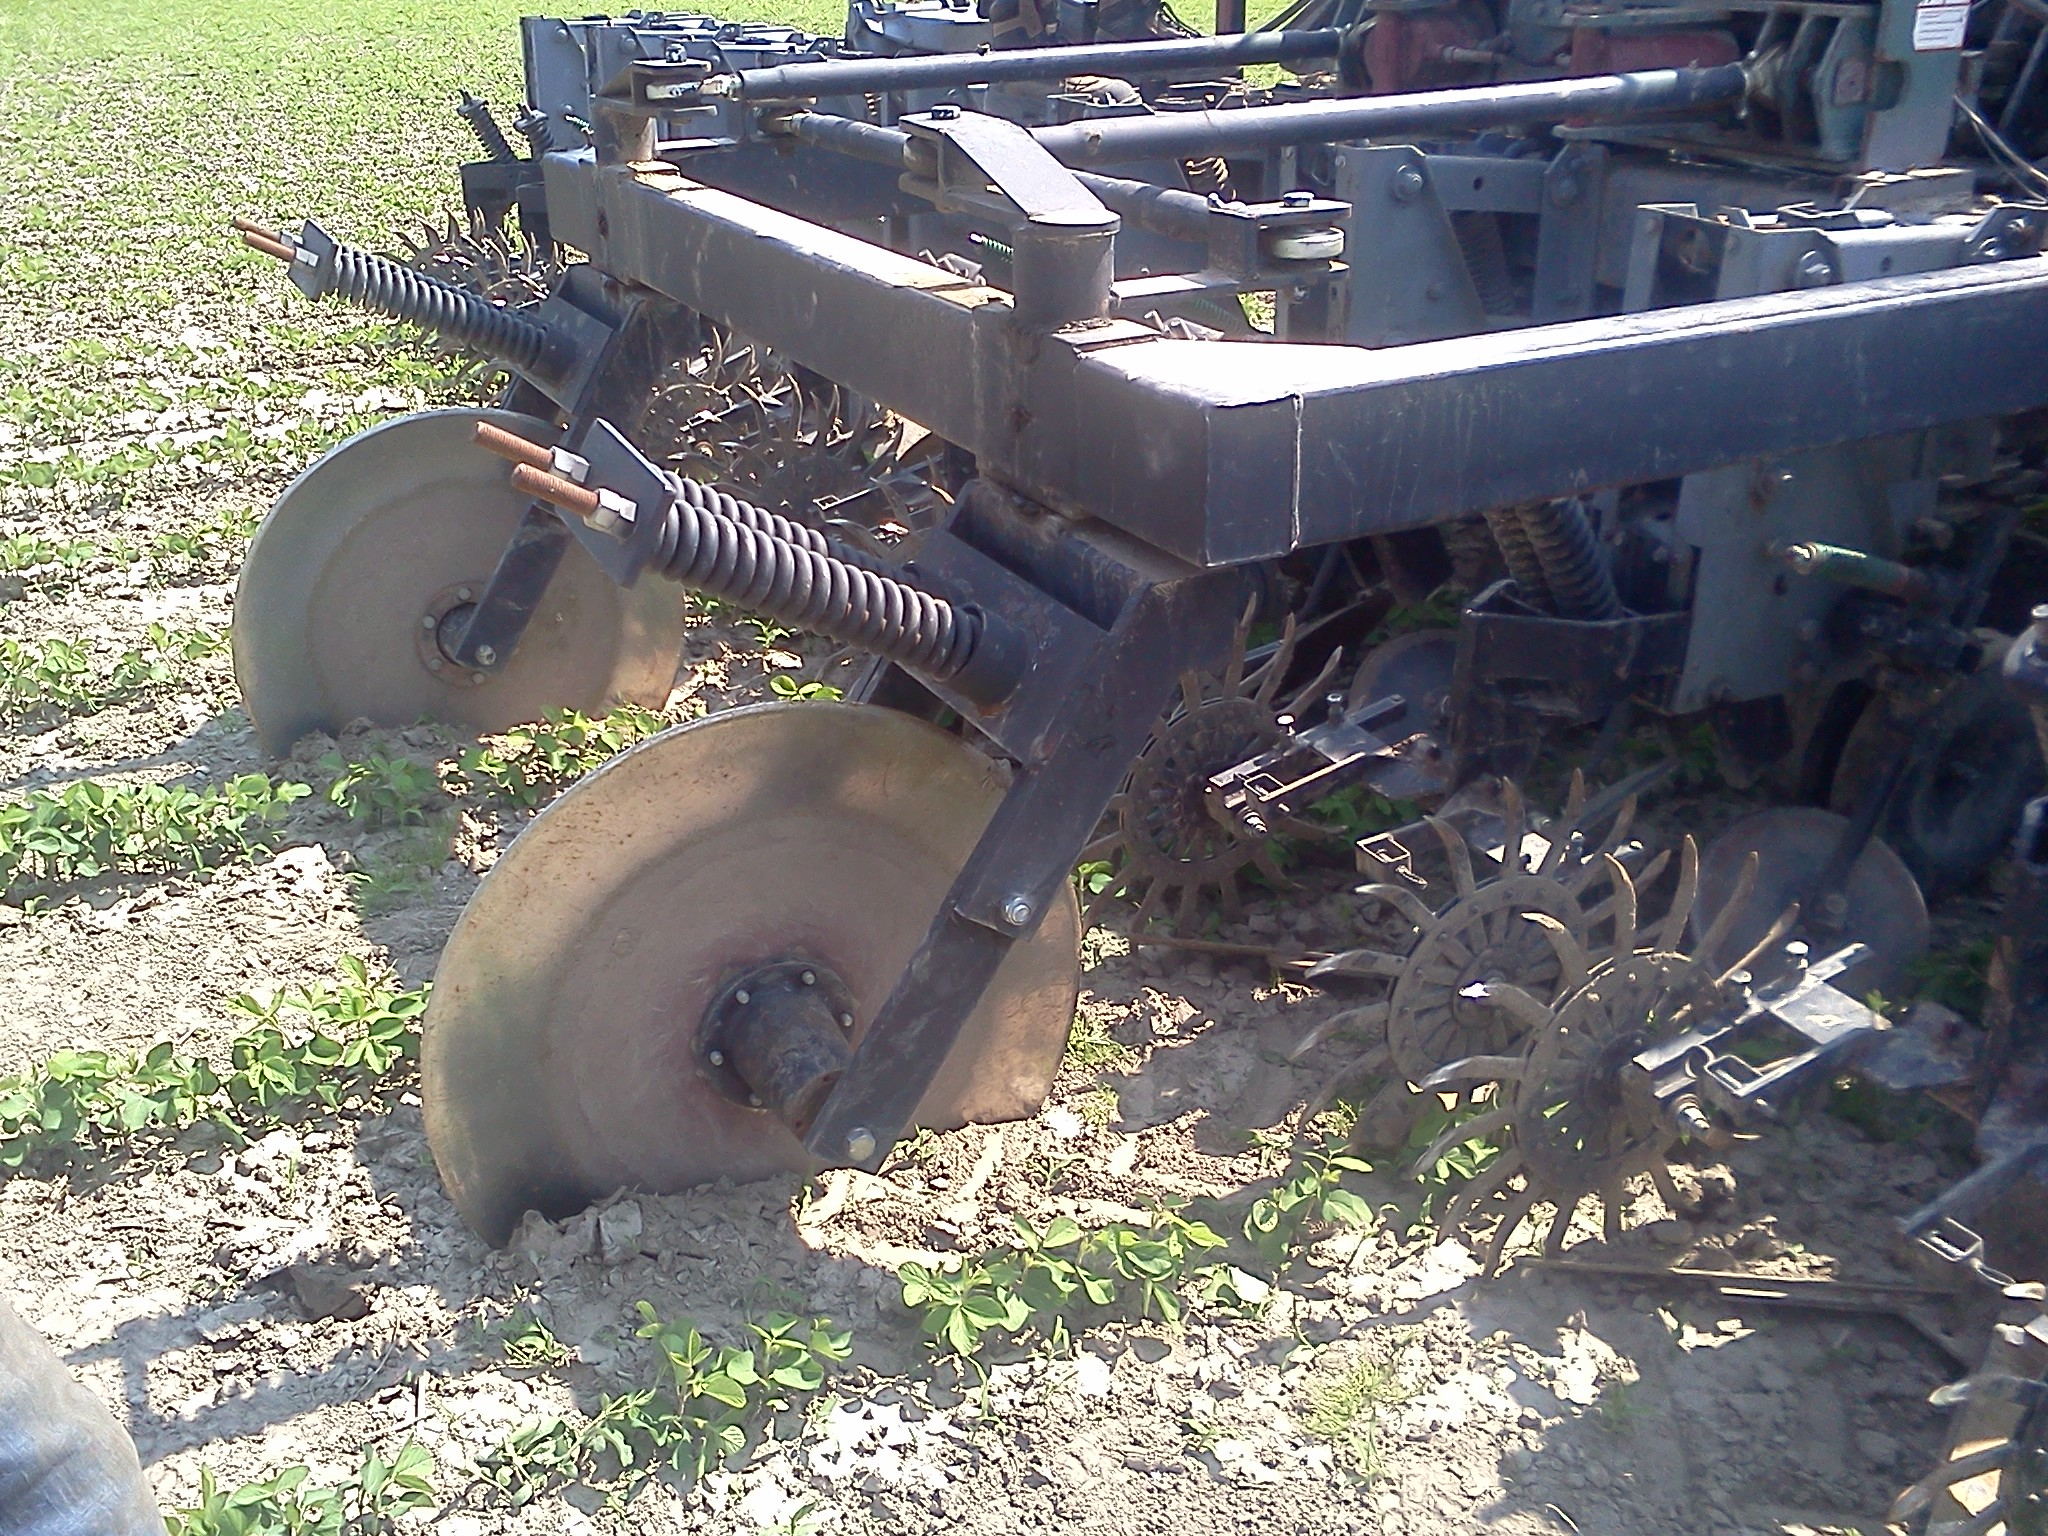
\includegraphics[scale=0.1,natwidth=610,natheight=642]{stabilizers.jpg}
  \caption{Rotating stabilizers}
  \label{fig:stabilizers}
\end{figure}

The output value was transmitted via a weatherproof (IP68) USB
connection to the microcontroller which was interfaced with the
hydraulic solenoid controller. The microcontroller generates an analog
output signal via pulse-width modulation (PWM) to produce a voltage
range from 0.0 V to 5.0$\pm$0.05 V. However, the operating range of the
Sukup Auto-Guide system is from 0.10$\pm$0.02V to 8.0$\pm$0.02V with a fixed
supply voltage of 9.70$\pm$0.02V. To account for this discrepancy, the PWM
output range was scaled linearly and a logic level converter (LLC)
circuit was used to rescale and shift the PWM signal to the required
range.

\begin{equation}
  w = 
  \begin{cases}
    0 & \quad \text{if } u \leq 0 \\
    2^{R-1} & \quad \text{if } u \geq 2^{R-1}\\
    (u +2^{R-2})\times\left[\frac{V_{max}}{V_{HV}}+\frac{V_{min}}{V_{LV}}\right] & \quad \text{else} \\
  \end{cases}
  \label{eq:v_out}
\end{equation}
\begin{flushleft}
where $V_{min}=0.10$, $V_{max}=8.00$, $V_{HV}=9.70$, $V_{LV}=5.0$
\end{flushleft}

\begin{equation}
  V_{hydraulic} = \frac{w}{2^{R-1}} \times V_{HV} + V_{min}
  \label{eq:v_out}
\end{equation}
\begin{flushleft}
where $V_{min}=0.10$, $V_{max}=8.00$, $V_{HV}=9.70$, $V_{LV}=5.0$
\end{flushleft}

To produce this output, a signal condition circuit was employed making
use of a MOSFET logici-level converter. This allows the system to
output a voltage using PWM to systems with different voltage
requirements.

\begin{figure}
  \centering
  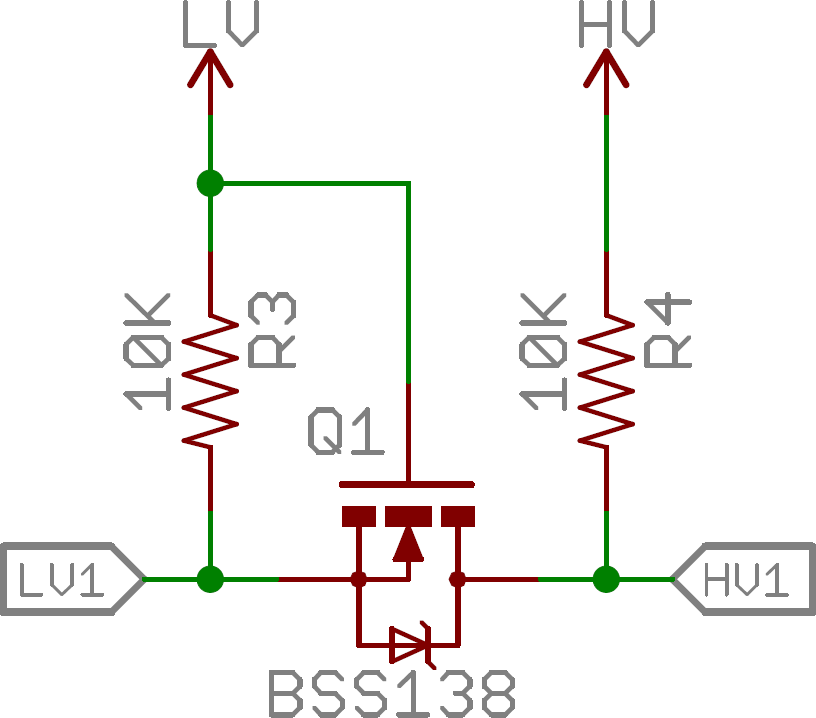
\includegraphics[scale=0.3,natwidth=610,natheight=642]{signal_conditioning.png}
  \caption{Rotating stabilizers}
  \label{fig:signal_conditioning}
\end{figure}

This final output voltage represents the desired set-point for angle
of the steering stabilizers to be reached by hydraulic solenoid
controller. The mapping between output voltage and position was found
to be a linear, second order system, with saturation.

\begin{equation}
  \frac{d^2}{dt^2}x + 2\zeta\omega_{n}\frac{d}{dt}x + \omega_{n}^2 Kx = 0 
  \label{eq:v_out}
\end{equation}
where $K=0.3275$ rad/V at a sensitivity setting of 10.

\subsection{Calibration}
At the beginning of each day of field trials, a camera calibration
procedure was followed to ensure proper alignment of the cameras: (1)
the cultivator was aligned with the crop rows which was verified by
measurements with a tape measure at the working tools; (2) lateral
adjustments were made to the camera bracket to ensure the vertical
center-line of each camera was aligned with the crop row; (3) vertical
adjustments made to the camera bracket to ensure a subject depth of
100 cm from the camera lens to the soil surface.

Additionally, the Sukup Auto-Guide system provides basic user tuning
in the form of sensitivity and tracking adjustment inputs. The
sensitivity adjustment effectively changes the mapping between voltage
and radial resolution of the stabilizers, with a range of 1 to 10
resulting in mappings from 0.1350 rad/V to 0.3275 rad/V,
respectively. Similarly, the tracking adjustment offsets the zero
position of the stabilizers on a scale of -3 to +3 corresponding to
-0.435 rad to +0.435 rad, respectively. Therefore, at the beginning of
each set of trials the following settings were ensured: (1) the
sensitivity was set to 10 out of 10, and (2) the tracking adjustment
was set to 0.

\subsection{Field Trials}
Field tests of the system took place over the summer of 2014 from June
to August on straight-drilled corn and soybean crops. Only organic
cultivars were considered for this study, therefore no pesticides were
applied to the fields and weeds were present during testing. All
fields used during testing were maintained by Agri-Fusion 2000 Inc., a
4000 ha organic farming operation in St-Polycarpe, Quebec. Trials were
classified into four stages of crop development: $\le$10 cm, 10 - 15
cm, 15 - 20 cm, and $\ge$20 cm. For each run, five representative
locations along the row were selected and the height of the crop from
the soil surface was observed using a tape measure, and the resulting
average determined the height stage of the trial. To determine the
reliability of the two systems at differing speeds of operation,
trials were conducted at four approximate travel speeds: 6, 8, 10, and
12 km/h. The travel speed of the tractor was set via the automatic
speed controller of the vehicle.

% --- END Methodology --- %

% % --- BEGIN Results --- %
\section{Results}

% --- BEGIN Summary Table --- %
\begin{table}[h]
  \centering
  \caption{Summary of all trials.} 
  \scalebox{0.6}{
    \begin{tabular}{lccccc}
      \toprule
      Treatment & Crop Stage & Travel Speed (km/h) & Duration (s) &
      RMSE (cm) & 95$^{th}$ (cm) \\
      \midrule
      Computer-vision
      & soy ($<$10 cm)
         & 6 & 476 & 1.5 & 2.6\\
      &  &   & 375 & 1.3 & 2.5\\
      &  &   &  71 & 1.7 & 3.8\\
      &  & 8 &  80 & 2.1 & 4.0\\
      &  & 10&  61 & 2.1 & 3.8\\
      &  &   &  50 & 1.4 & 2.4\\
      \cmidrule(1r){2-6}
      & soy (10$-$15 cm)
         & 6 & 313 & 1.0 & 1.8\\
      &  & 8 & 360 & 1.8 & 2.8\\
      &  &   & 313 & 1.6 & 2.8\\
      &  &   & 139 & 3.6 & 7.0\\
      &  & 10& 380 & 1.5 & 3.0\\
      &  & 12& 418 & 1.7 & 2.8\\
      \cmidrule(1r){2-6}
      & soy ($>$15 cm)
         & 8 & 437 & 2.5 & 3.4\\
      &  & 10& 360 & 2.1 & 3.0\\
      &  & 12& 353 & 1.7 & 3.0\\
      &  &   &  98 & 2.5 & 3.6\\
      &  &   & 298 & 2.8 & 5.4\\
      &  &   & 205 & 1.9 & 3.4\\
      \cmidrule(1r){2-6}
      & corn ($\ge$15 cm)
         & 6 & 55  & 1.7 & 3.0\\
      &  & 8 & 81  & 4.3 & 5.2\\
      &  &   & 112 & 1.5 & 3.0\\
      &  &   & 140 & 1.9 & 3.6\\
      &  & 10& 189 & 1.7 & 3.4\\
      &  &   & 225 & 1.7 & 3.0\\
      &  & 12& 193 & 2.2 & 4.0\\
      \midrule
      Guiding rods
      & soy ($<$10 cm)
         & 6 & 58  & 2.6 & 4.6\\
      &  &   & 76  & 3.5 & 6.6\\
      &  & 8 & 84  & 3.4 & 7.0\\
      &  &   & 84  & 3.5 & 5.6\\
      &  & 10& 101 & 5.0 & 10.2\\
      \cmidrule(1r){2-6}
      & soy (10$-$15 cm)
         & 8 & 140 & 3.2 & 5.8\\
      &  &   & 100 & 4.2 & 7.0\\
      &  & 10& 145 & 2.9 & 6.0\\
      &  &   & 138 & 4.6 & 8.4\\
      &  & 12& 96  & 5.0 & 9.8\\
      \cmidrule(1r){2-6}
      & soy ($>$15 cm)
         & 6 & 556 & 2.0 & 4.0\\
      &  &   & 625 & 1.0 & 2.4\\
      &  & 10& 344 & 1.5 & 2.4\\
      &  &   & 156 & 1.3 & 2.8\\
      &  & 12& 107 & 1.7 & 3.0\\
      &  &   & 146 & 2.8 & 6.2\\
      &  &   & 104 & 1.4 & 2.6\\
      &  &   & 153 & 1.9 & 3.0\\
      \cmidrule(1r){2-6}
      & corn ($\ge$15 cm)
         & 6 & 167 & 1.6 & 3.0\\
      &  &   & 338 & 3.7 & 6.8\\
      &  & 8 & 195 & 2.0 & 3.8 \\
      &  &   & 211 & 1.7 & 3.0\\
      &  & 10& 274 & 2.0 & 3.8\\
      &  & 12& 128 & 2.3 & 4.4\\
      \bottomrule
    \end{tabular}
  }
  \label{table:all_trials}
\end{table}
% --- END Summary Table --- %

% --- BEGIN Crop Stage --- %
\begin{table}[h]
  \centering
  \caption{RMSE and 95$^{th}$ Percentile
    with respect to crop-stage.} 
  \scalebox{0.6}{
    \begin{tabular}{lcccccccc}
      \toprule
      \multirow{2}[10]{*} & \multicolumn{4}{c}{RMSE (cm)} &
      \multicolumn{4}{c}{95$^{th}$ Percentile (cm)} \\
      \cmidrule(1r){2-5} \cmidrule(1r){6-9}  
      & soy ($\le$10 cm) & soy (10$-$15 cm) & soy ($>$15 cm) &  corn ($\ge$15 cm) & soy ($\le$10 cm) & soy (10$-$15 cm) & soy ($>$15 cm) &  corn ($\ge$15 cm) \\
      \midrule
      Computer-vision & 1.70 $\pm$ 0.36 & 1.87 $\pm$ 0.91 & 2.22 $\pm$ 0.41 & 2.15 $\pm$ 0.99 & 3.18 $\pm$ 0.76 & 3.37 $\pm$ 1.83 & 3.63 $\pm$ 0.90 & 3.60 $\pm$ 0.8 \\
      Guiding rods & 3.61 $\pm$ 0.86 & 3.98 $\pm$ 0.89 & 1.70 $\pm$ 0.55 & 2.22 $\pm$ 0.78 & 6.8 $\pm$ 2.12 & 7.40 $\pm$ 1.69 & 3.30 $\pm$ 1.28 & 4.13 $\pm$ 1.41 \\
      \bottomrule
    \end{tabular}
  }
  \label{table:travel_speed}
\end{table}
% --- END Crop Stage Table --- %

% --- BEGIN Tukey Table --- %
\begin{table}[h]
  \centering
  \caption{Tukey multiple comparison of $95^{th}$ percentiles, $\alpha=0.05$} 
  \scalebox{0.8}{
    \begin{tabular}{lcccccccc}
      \toprule
      Computer-vision & Guiding rods & Mean (cm) & Lower (cm) & Upper (cm) & Accept \\
      \midrule
      corn $>$15 & \multicolumn{1}{l}{corn $\ge$15} &  0.06 &  -1.28 & 1.40 &False \\
      corn $>$15 & \multicolumn{1}{l}{soy $<$10}   &  1.74 &   0.45 & 3.02  & True \\
      corn $>$15 & \multicolumn{1}{l}{soy 10$-$15} &  1.41 &  -0.24 & 3.07 &False \\
      corn $>$15 & \multicolumn{1}{l}{soy $>$15}   & -0.45 &  -1.70 & 0.79 &False \\
      soy $<$10  & \multicolumn{1}{l}{corn $>$15}  &  0.86 &  -0.41 & 2.12& False \\
      soy $<$10  & \multicolumn{1}{l}{soy $<$10}   & 2.53  &   1.32   &3.74  & True \\
      soy $<$10  & \multicolumn{1}{l}{soy 10$-$15} & 2.21  &  0.61  &3.81 & True \\
      soy $<$10  & \multicolumn{1}{l}{soy $>$15}   & 0.34  & -0.83  &1.51 &False \\
      soy 10$-$15& \multicolumn{1}{l}{corn $\ge$15}&  0.35 &  -1.04 & 1.73 & False \\
      soy 10$-$15& \multicolumn{1}{l}{soy $<$10}   & 2.02  &  0.68  & 3.36 & True \\
      soy 10$-$15& \multicolumn{1}{l}{soy 10$<$15} &  1.70 &  0.00  &3.40 & True \\
      soy 10$-$15& \multicolumn{1}{l}{soy $>$15}   & -0.17 &  -1.47 & 1.13 & False \\
      soy $>$15  & \multicolumn{1}{l}{corn $\ge$15}& -0.01 & -1.40  &1.38 & False \\
      soy $>$15  & \multicolumn{1}{l}{soy $<$10}   & 1.67  &  0.33  &3.00  & True \\
      soy $>$15  & \multicolumn{1}{l}{soy 10$-$15} & 1.35  & -0.35 & 3.04 &False \\
      soy $>$15  & \multicolumn{1}{l}{soy $>$15}   & -0.52 &  -1.82 & 0.77 &False \\
      \bottomrule
    \end{tabular}
  }
  \label{table:tukey}
\end{table}
% --- END Tukey Table --- %

% --- END Results --- %

% --- BEGIN Discussion --- %
\section{Discussion}
With respect to RMSE, the two systems performed comparatively, with an
average RMSE of less than 3.5 cm for both the computer-vision and the
guiding rod systems for all crop stages \ref{table:travel_speed}. However, with
respect to the 95th percentile, the guiding rods resulted in
greater error than the computer-vision system for crops at the $\le$10
cm and 10-15 cm stages (Table \ref{table:tukey}). Comparatively, the computer-vision
system had an average 95th percentile of $\le$3.8 cm for all four
crop stages with the exception of one trial. The accuracy of the guiding rods increased dramatically
as the plants matured, resulting in a significant decline in average
95th percentile and average RMSE at the 15-20 cm and $\ge$20 cm
stages. The computer-vision system showed significantly lower error
than the guiding rods for crop stages less than 20 cm in height, but a
slight increase in error for plants greater than 20 cm. 

There was no apparent correlation between error and travel speed for
both systems, either with respect to RMSE or 95th percentile. Notably,
the computer vision guidance system outperformed the mechanical system
at all travel speeds; however, this affect is likely due to the
interaction with crop height, not travel speed.

\subsection{Future Improvements}
Due to the fact that the cameras used for this study were intended for
security applications, the cameras were designed for usage in a wide
range of ambient lighting. Specifically, the photosensor of the
cameras was sensitive to infrared (IR) light and featured a built-in
array of 24 IR LEDs. Although this feature theoretically extended the
daily hours of operation, IR-sensitivity proved to have a negative
affect on color-quality under intense ambient light, i.e. $\ge$20000 Lux,
resulting in over-exposure and blue-shifting of green tones in the HSV
color-space. To correct for this effect, applying contrast-limited adaptive
histogram equalization (CLAHE) as a pre-processing technique prior to the BPPD
filter may reduce the negative affects of IR-sensitivity without
requiring hardware changes (e.g. non-IR sensitive cameras or usage of
an IR filtering lens).

In this study, since row offsets were determined by analyzing the
plant foliage mask in the direction of travel with a relatively small
subject distance, no perspective or radial distortion correction was
implemented. However for alternate 
usage cases, e.g. cameras aligned at the mid-point between rows, it
would be necessary for perspective and lens-distortion correction to
be implemented. Due to the nature of how these systems are installed,
a versatile method for in-field camera calibration demonstrated by
\citet{lee2002} can be utilized. This method utilizes a
checkerboard pattern which is placed in the camera’s field of view. An
image is captured and the positions of the corners are
identified. Using the known size of the squares, the calibration
coefficients can be calculated which can be used on new images to
rectilinearize the image, thus correcting for perspective and radial
distortion.

\begin{figure}
  \centering
  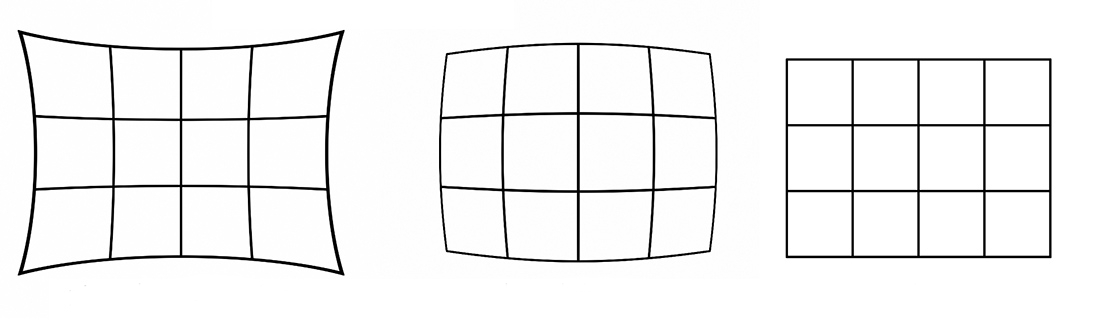
\includegraphics[width=0.8\textwidth,natwidth=610,natheight=642]{lens_distortion.jpg}
  \caption{Lens distortion}
  \label{fig:distortion}
\end{figure}

With respect to the hydraulic steering system, this study was limited
to a rotating stabilizer implement guidance system
and therefore the orientation of the crop rows relative to the
cultivator (and by extension the cameras) was effectively
orthogonal. As such, the method for row detection using histogram
analysis in the direction of travel is appropriate for both rotating
stabilizer and center-shift steering systems. However several
commercially available hydraulic steering system designs make use of
pivoting hitch systems. In such systems, the cultivator toolbar is
rotated about a central pivot point to generate the lateral adjustment
force (\ref{fig:pivoting_hitch}).

\begin{figure}
  \centering
  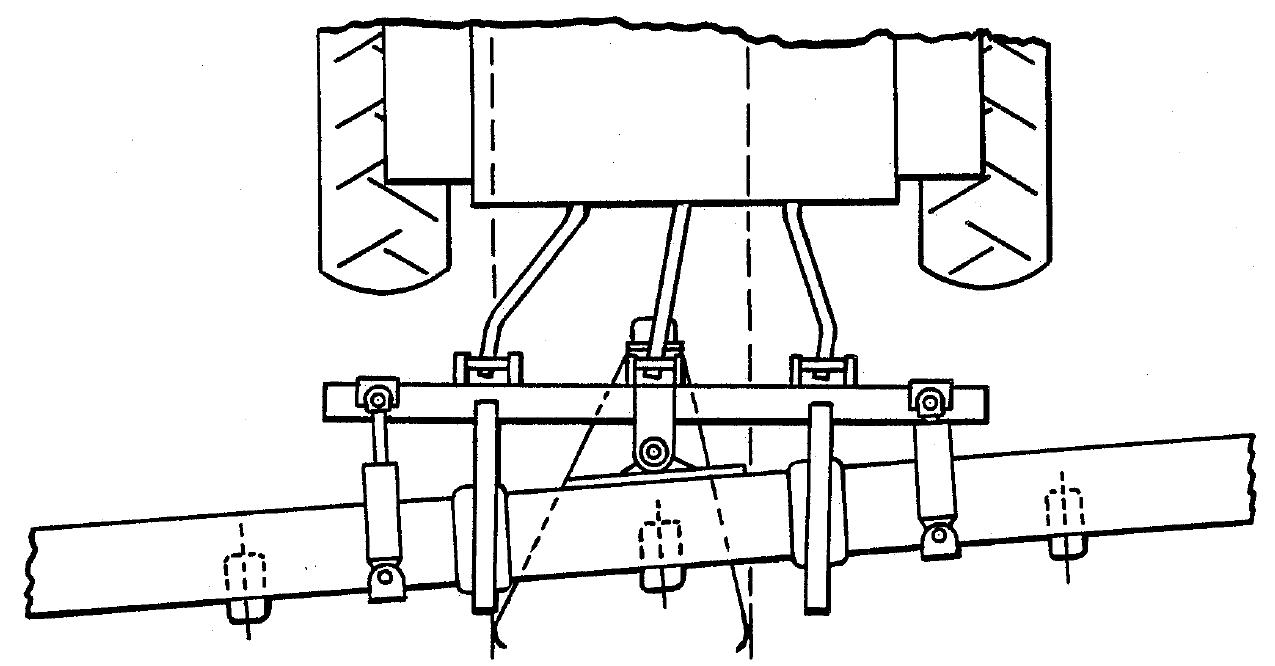
\includegraphics[width=0.8\textwidth,natwidth=610,natheight=642]{pivoting_hitch.png}
  \caption{Pivoting hitch hydraulic steering system.}
  \label{fig:pivoting_hitch}
\end{figure}

Pivoting hitch steering systems may rotate the cultivator toolbar as
much as $\pm5$ degrees. This pivoting action effectively changes the
apparent offset of the crop row (Equation \ref{eq:pivot_error}), and
therefore would significantly reduce the accuracy of row estimation
using the method proposed in this paper. To compensate for this
effect, knowledge of the camera's position relative to the pivot point
is required ($x_0$ and $y_0$) as well as the camera's instantaneous
orientation relative to the direction of travel ($\theta_0$). Although
the hitch's angle of orientation could be determined via sensor
feedback from the hitch itself (e.g. via rotary encoder), an
alternative approach using computer-vision is also an attractive
option. Methods such the Hough Line Transform or feature-based motion
estimation of the images (i.e. keypoint tracking) may be proove to be
robust solutions which do not require integration with the hitch
controller and would therefore be system-agnostic.

\begin{equation}
  \begin{split}
  \epsilon_x = x_0 - \sqrt{x_0^2 + y_0^2} \times sin\left(\theta -
  tan^{-1}(\frac{y_0}{x_0})\right) \\
  \epsilon_y = y_0 - \sqrt{x_0^2 + y_0^2} \times cos\left(\theta -
  tan^{-1}(\frac{y_0}{x_0})\right)
  \end{split}
  \label{eq:pivot_error}
\end{equation}
\begin{flushleft}
where $x_0$ is the lateral distance from the camera to the pivot
point, $y_0$ is the loongitudinal distance from the camera to the pivot
point, and $\theta$ is the instantaneous orientation of the camera relative to the
direction of travel.
\end{flushleft}

Due to the method of integrating computer-vision into an existing
hydraulic steering controller, manual adjustments are available to the
operator via a control panel, allowing the operator to manually override the
offset and sensitivity of the guidance system. For such a
steering system there exist several uncontrollable variables which can
have a detrimental impact on the performance, e.g. soil conditions,
terrain slope, tractor pulling power, and travel speed. To account for
this inherent non-linearity and variability of implement steering,
dynamic learning is a possible solution which does not require regular human
intervention. Real-time reinforcement learning techniques, such as
Q-learning, may be very applicable to this style of control
system. The Q-learning algorithm is primarilty intended applications
with uncalibrated control of non-linear, multiple input, multiple output systems. 
Q-learning functions on the principal that at any given
moment the behavior of the system can be assessed and subsequently
rewarded or penalized. Therefore, over-time actions which result
in positive behavior for a given state of the system (e.g. high gain
when drifting away from the target) are incentivized and those which
resulted in negative behavior (e.g. high gains resulting in
overshooting target) are penalized. Ultimately, the learning process
produces a non-linear response matrix which adapts to the current
working environment of the system.

\begin{equation}
  Q_{t+1}(s_t,a_t) = Q_{t}(s_t,a_t) + \alpha_{t}(s_t,a_t) \times
  \left( R_{t+1} + \gamma \times Q_{} \right)
  \label{eq:qlearning}
\end{equation}
\begin{flushleft}
where $Q$ is the cost matrix, $s$ is the current state, and $\alpha$
is the learning rate. 
\end{flushleft}
% --- END Discussion --- %

% --- BEGIN Conclusion --- %
\section{Conclusion}
The BPPD method performed well in various lighting conditions and crop conditions.
The computer-vision system achieved an average 95th percentile of <
4.0 cm for all crop stages, and significantly outperformed the guiding
rods at the earliest stages of growth, i.e. <10 cm and 10-15 cm. However, at
later stages of growth (>15 cm) there was no observable difference in
performance between the two guidance systems. 

\subsection{Acknowledgements}
This study was supported in part by funding provided through the
National Science and Engineering Research of Canada (NSERC) Engage
program with assistance from Jean Cantin of the Quebec Ministry of
Agriculture, Fisheries and Food (MAPAQ).
% --- END Conclusion --- %

\section{References}
\bibliography{references.bib}

\end{document}
% --- END  --- %